\documentclass[tikz,border=8pt]{standalone}
\usepackage{amsmath}
\usetikzlibrary{arrows.meta,positioning,calc}
\definecolor{ink}{HTML}{21352F}\definecolor{teal}{HTML}{087F7B}\definecolor{gold}{HTML}{C58B2A}\definecolor{rose}{HTML}{B65A62}
\begin{document}
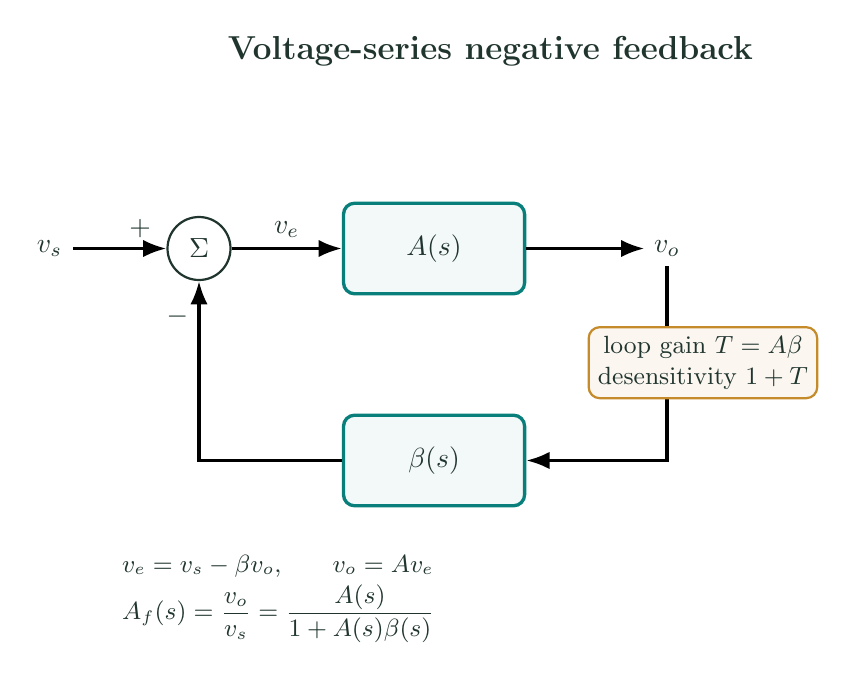
\begin{tikzpicture}[font=\sffamily,text=ink,>=Latex,block/.style={draw=teal,very thick,rounded corners,minimum width=2.3cm,minimum height=1.15cm,fill=teal!5},sum/.style={draw=ink,thick,circle,minimum size=8mm}]
 \node[font=\bfseries\large] at (3.7,2.5) {Voltage-series negative feedback};
 \node (s) [sum] at (0,0) {$\Sigma$};
 \node[block,right=1.4cm of s] (a) {$A(s)$};
 \node[right=1.5cm of a] (o) {$v_o$};
 \node[block,below=1.5cm of a] (b) {$\beta(s)$};
 \draw[->,very thick] (-1.6,0) node[left]{$v_s$} -- (s) node[pos=.72,above]{$+$};
 \draw[->,very thick] (s)-- node[above]{$v_e$}(a);
 \draw[->,very thick] (a)--(o);
 \draw[->,very thick] (o)|-(b.east);
 \draw[->,very thick] (b.west)-|(s.south) node[pos=.9,left]{$-$};
 \node[anchor=west,align=left,font=\small] at (-1.1,-4.45) {$v_e=v_s-\beta v_o$,\qquad $v_o=A v_e$\\[2pt]$\displaystyle A_f(s)=\frac{v_o}{v_s}=\frac{A(s)}{1+A(s)\beta(s)}$};
 \node[draw=gold,thick,rounded corners,fill=gold!7,align=center,font=\small] at (6.4,-1.45) {loop gain $T=A\beta$\\desensitivity $1+T$};
\end{tikzpicture}
\end{document}
